% Options for packages loaded elsewhere
\PassOptionsToPackage{unicode}{hyperref}
\PassOptionsToPackage{hyphens}{url}
%
\documentclass[
]{article}
\usepackage{amsmath,amssymb}
\usepackage{lmodern}
\usepackage{ifxetex,ifluatex}
\ifnum 0\ifxetex 1\fi\ifluatex 1\fi=0 % if pdftex
  \usepackage[T1]{fontenc}
  \usepackage[utf8]{inputenc}
  \usepackage{textcomp} % provide euro and other symbols
\else % if luatex or xetex
  \usepackage{unicode-math}
  \defaultfontfeatures{Scale=MatchLowercase}
  \defaultfontfeatures[\rmfamily]{Ligatures=TeX,Scale=1}
\fi
% Use upquote if available, for straight quotes in verbatim environments
\IfFileExists{upquote.sty}{\usepackage{upquote}}{}
\IfFileExists{microtype.sty}{% use microtype if available
  \usepackage[]{microtype}
  \UseMicrotypeSet[protrusion]{basicmath} % disable protrusion for tt fonts
}{}
\makeatletter
\@ifundefined{KOMAClassName}{% if non-KOMA class
  \IfFileExists{parskip.sty}{%
    \usepackage{parskip}
  }{% else
    \setlength{\parindent}{0pt}
    \setlength{\parskip}{6pt plus 2pt minus 1pt}}
}{% if KOMA class
  \KOMAoptions{parskip=half}}
\makeatother
\usepackage{xcolor}
\IfFileExists{xurl.sty}{\usepackage{xurl}}{} % add URL line breaks if available
\IfFileExists{bookmark.sty}{\usepackage{bookmark}}{\usepackage{hyperref}}
\hypersetup{
  pdftitle={First Markdown Assignment v.0.03},
  hidelinks,
  pdfcreator={LaTeX via pandoc}}
\urlstyle{same} % disable monospaced font for URLs
\usepackage[margin=1in]{geometry}
\usepackage{graphicx}
\makeatletter
\def\maxwidth{\ifdim\Gin@nat@width>\linewidth\linewidth\else\Gin@nat@width\fi}
\def\maxheight{\ifdim\Gin@nat@height>\textheight\textheight\else\Gin@nat@height\fi}
\makeatother
% Scale images if necessary, so that they will not overflow the page
% margins by default, and it is still possible to overwrite the defaults
% using explicit options in \includegraphics[width, height, ...]{}
\setkeys{Gin}{width=\maxwidth,height=\maxheight,keepaspectratio}
% Set default figure placement to htbp
\makeatletter
\def\fps@figure{htbp}
\makeatother
\setlength{\emergencystretch}{3em} % prevent overfull lines
\providecommand{\tightlist}{%
  \setlength{\itemsep}{0pt}\setlength{\parskip}{0pt}}
\setcounter{secnumdepth}{-\maxdimen} % remove section numbering
\ifluatex
  \usepackage{selnolig}  % disable illegal ligatures
\fi

\title{First Markdown Assignment v.0.03}
\author{}
\date{\vspace{-2.5em}}

\begin{document}
\maketitle

\hypertarget{question-1}{%
\subsubsection{\texorpdfstring{\textbf{Question
1:}}{Question 1:}}\label{question-1}}

\hypertarget{aside-from-reasons-mentioned-above-why-do-we-need-to-study-and-analyze-data}{%
\paragraph{Aside from reasons mentioned above, why do we need to study
and analyze
data?}\label{aside-from-reasons-mentioned-above-why-do-we-need-to-study-and-analyze-data}}

\textbf{Data analysis} is \emph{an important process to make the right
decisions.} When one began to gather and analyze data, one will likely
find it easier to reach a particular decision to make (Business
Insights, 2019). With the use of data analysis, a complex and abstract
problem is being simplified into series of small problems that can now
be solved with the help of available data. The options are now being
weighed based on different criteria that one has set to satisfy his own
wants and needs. Because data is available everywhere and we acquire it
every day, we started to look for patterns to make sense of the
scattered data available.

\begin{figure}
\centering
\includegraphics{https://d2slcw3kip6qmk.cloudfront.net/marketing/blog/2018Q2/critical-elements-for-decision-making/operations-webinar-recap-header@2x.png}
\caption{Critical Elements for Decision Making}
\end{figure}

Data science is \emph{being used as a tool to communicate with a certain
group of people}, thus, it \emph{helps in improving people's lives.}
This should be the main goal of a certain organization in obtaining and
collecting data to design different tools that will help in improving
people's lives. Also, the use of data science allows organizations and
individuals to more effectively determine the cause of the problem. With
the help of data analysis, one will be able to visualize and determine
striking relationships between circumstances that they encountered. When
the problems have been pointed out, they will be able to strategize
approaches in solving a particular problem that will increase their
efficiency. Data analysis helps an individual and an organization to
determine which should take priority over the others (The Council on
Quality and Leadership, n.d.).

\includegraphics{https://edexec.co.uk/wp-content/uploads/2017/06/Have-your-say-comment.jpg}
Data science is a valuable field of study because the vast amounts of
raw data acquirable online and in person is just ``white noise'' that
makes little sense to anyone who isn't a statistician. It is up to the
people who study data science to make sense of this data and present it
in ways that allow the general public to understand and make use of this
data.

Data interpretation and analysis is a significant aspect when we work
with data sets in any field we are in. As we analyze data, it becomes
helpful for us to acquire useful and relevant information from a lot of
unorganized data that will enable us to arrive at a solid decision that
is not only useful for businesses and researchers, but also for
individuals.

\textbf{References:}

12 reasons why data is important. (n.d.). The Council on Quality and
Leadership. Retrieved July 9, 2021, from
\url{https://www.c-q-l.org/resources/guides/12-reasons-why-data-is-important/}

The advantages of data-driven decision-making. (2019, August 26).
Business Insights - Blog.
\url{https://online.hbs.edu/blog/post/data-driven-decision-making}

\begin{center}\rule{0.5\linewidth}{0.5pt}\end{center}

\hypertarget{question-2}{%
\subsubsection{\texorpdfstring{\textbf{Question
2:}}{Question 2:}}\label{question-2}}

\hypertarget{cite-atleast-one-instance-or-application-where-data-science-was-used-and-contributed-on-policy-making-day-to-day-decisions-knowing-market-trends-and-scientific-researches.}{%
\paragraph{Cite atleast one instance or application where data science
was used and contributed on policy-making, day-to-day decisions, knowing
market trends, and scientific
researches.}\label{cite-atleast-one-instance-or-application-where-data-science-was-used-and-contributed-on-policy-making-day-to-day-decisions-knowing-market-trends-and-scientific-researches.}}

One of the applications of data science in everyday life is \textbf{data
personalization by a person's preferences} in entertainment websites or
apps such as \emph{Spotify} and \emph{Netflix}. Netflix programming uses
algorithms that are designed to produce shows, and then catered to their
consumers whose behavior patterns suggest that they might like their
programming that came from their databases. This allows them to
customize the watchlist of their consumers in accordance with popular
actors, genre, or just through consumer preference (Jahnke, 2019).
Meanwhile, similar to Netflix, Spotify also uses data in order to
customize their weekly playlist of songs that again, cater to the
preferences of their consumers. Through modern data science
technologies, not only do the users of these entertainment apps or
websites get entertained, but also allows the distributors to save lots
of money that once would have been spent on marketing. It also allows
these distributors not only to acquire the licensing of certain content
from other distributors to satisfy their consumers but also to
``create'' content themselves (such as the Netflix original series
Stranger Things) because they know what their consumers would like.

\begin{figure}
\centering
\includegraphics{https://drupal.anyforsoft.com/sites/default/files/inline-images/netflix-ai-trend.jpg}
\caption{Netflix recommendations}
\end{figure}

Another application of data science is in the \textbf{healthcare
industry}. It plays a very important role in monitoring a patient's
health and notifying necessary steps to be taken in order to detect
potential diseases in order to prevent them from taking place. This
proved to be very beneficial as a late detection of any disease would
not only be detrimental to a person's health but it would also cost them
a lot of money to treat the disease or ailment (Data Flair, 2021). Data
science also helps in monitoring a patient's health. Wearable devices
that track heartbeat, temperature and other medical parameters collect
data that would be soon analyzed by doctors or/and medical experts to
not only detect any sign of ailment or disease but also to keep track of
a patient's blood pressure, calorie intake and many others. These
devices use real-time analytics to predict any problem based on the
patient's present condition, which helps doctors assess the necessary
conditions to help patients in distress.

\includegraphics{https://techvidvan.com/tutorials/wp-content/uploads/sites/2/2020/02/Data-Science-in-Healthcare-1.jpg}
Another instance of data science contributing to change is the many
different statistics that are used in gauging the effects of global
warming. Massive amounts of data gathered by scientists around the world
about the ever changing environment are used as a basis on sanctioning
harmful industries and practices, all for the sake of the environment.

\begin{figure}
\centering
\includegraphics{https://ccimgs-2019.s3.amazonaws.com/2019DecadeTemps/2019DecadeTemps_Global_C_en_title_lg.jpg}
\caption{Global Warming}
\end{figure}

Finally, another notable application of data science is in the
\textbf{Finance sector}. Banks can now easily manage massive amounts of
data to learn more about their clients so that they could drive new
revenue opportunities and improve their business decision making.
Another is an effective customer support service. Clients could just
easily contact a customer service representative through landline or
through the internet (via email and voice chat or call), which enables
them to ask questions or send complaints without the need (or at least
limits the necessity) to personally go to a bank. It also enables
clients to ``pay online'' or ``contactless payment'' which enables their
clients to shop online through the use of a credit or debit card.
Finally, through data science, banks can safely handle and keep track of
their clients accounts to avoid credit card fraud, the breach of
important financial data, and any other suspicious activity that would
compromise their clients' financial accounts (Activewizards, n.d).

\begin{figure}
\centering
\includegraphics{https://data-flair.training/blogs/wp-content/uploads/sites/2/2019/04/data-science-in-Banking.jpg}
\caption{Data Scinece in Banking}
\end{figure}

\textbf{References:}

Data Flair (2021, April 02). Data Science in Healthcare - 7 Applications
No one will Tell You. Retrieved July 08, 2021, from
\url{https://data-flair.training/blogs/data-science-in-healthcare/}

Jahnke, A. (2019, March 07). Netflix, Spotify, and how data is shaping
the arts. Retrieved July 08, 2021, from
\url{https://www.bu.edu/articles/2019/data-arts/}

Activewizards (n.d.) Top 9 data science use cases in banking. Retrieved
July 09, 2021, from
\url{https://activewizards.com/blog/top-9-data-science-use-cases-in-banking/}

\begin{center}\rule{0.5\linewidth}{0.5pt}\end{center}

\hypertarget{question-3}{%
\subsubsection{\texorpdfstring{\textbf{Question
3:}}{Question 3:}}\label{question-3}}

\hypertarget{propose-atleast-one-data-science-topic-that-you-want-to-pursue-have-a-broad-description-of-the-topic-describe-the-availability-of-the-data-what-kinds-of-statistical-method-you-think-you-will-need-and-who-would-benefit-this-study.}{%
\paragraph{Propose atleast one data science topic that you want to
pursue: Have a broad description of the topic, describe the availability
of the data, what kinds of statistical method you think you will need,
and who would benefit this
study.}\label{propose-atleast-one-data-science-topic-that-you-want-to-pursue-have-a-broad-description-of-the-topic-describe-the-availability-of-the-data-what-kinds-of-statistical-method-you-think-you-will-need-and-who-would-benefit-this-study.}}

\hypertarget{salvador-lester-niel-s.}{%
\paragraph{Salvador, Lester Niel S.}\label{salvador-lester-niel-s.}}

The pandemic has brought us lots of challenges that made us look for
ways on how to survive the economic regression. A lot of Filipinos have
started their own small businesses such as online thrift shops, foods,
and many more. Because of this, I became interested in the growth of
Micro, Small, and Medium Enterprises (MSMEs) in the Philippines. Big
businesses are the ones who may control the stock market, but it is the
small businesses and start ups that keep the economy moving. Small
businesses are commonly found in the local barangays and places, thus,
generating more jobs and opportunities for local individuals. Small
businesses also have great potential because it is more often started by
individuals who have great ideas and aims to bring innovation and
something new in the industry.

This topic is timely and relevant to what the country is experiencing
and it becomes more interesting on how people are dealing with the lack
of jobs and worsening economy by establishing their own small
businesses. We can gather data from the website of the Department of
Trade and Industry for the number of small businesses established for
2018-2019, the United Nations Philippines official website, and other
studies about the growth of MSMEs in the Philippines more especially in
the time of the pandemic.

The statistical methods that we will be using for this study would be
numerical analysis of pre-existing data from reliable sources, data
management, and making generalizations and conclusions based on the data
that we have gathered. The main group of people who will benefit from
this study is those who have plans in starting their own businesses in
the middle of the pandemic and existing MSME owners so they can devise
their own plans for the betterment of their business.

\begin{figure}
\centering
\includegraphics{https://cannabrew.uk/wp-content/uploads/2021/01/small-business-saturday___17150639833.jpg}
\caption{Small Business}
\end{figure}

\hypertarget{sison-justine-matthew}{%
\paragraph{Sison, Justine Matthew}\label{sison-justine-matthew}}

One possible data science topic we could pursue is to determine the
unemployment rate of people in Metro Manila during the pandemic. Many
businesses had closed down and many companies laid off some if not most
of their workers to minimize their spending due to the lockdown where
their consumers had drastically reduced, thus having little to no
revenue. Because of that, there should be an increase in the
unemployment rate, but we would like to determine at what percentage the
unemployment rate increased when compared to 2019, the year before 2020
where the pandemic began. Since the country is vast, we decided to focus
on the unemployment rate here in Metro Manila, one of the most, if not
the most, urban cities in the country where most of the country's local
labor force are situated. However, the population in Metro Manila is
very populous, where according to world population review, the estimated
population in Metro Manila is about 14 million (World Population Review,
2021). Not to mention that we have very limited means to conduct a
survey with a very large sample size due to the limitations imposed by
the government and other limitations during the pandemic.

\begin{figure}
\centering
\includegraphics{https://media.philstar.com/photos/2020/09/03/july-jobless-01_2020-09-03_12-16-35_gallery.png}
\caption{2020 Unemployment rate in Metro Manila}
\end{figure}

Therefore, we would like to conduct a survey with a Stratified Random
Sampling as a means to determine the unemployment rate in Metro Manila.
We would like to get 25 respondents from each of the 17 municipalities
in Metro Manila, which would give us a total of 425 respondents.
Although it would be better if we have a larger sample size, we felt
that we cannot conduct a survey with more than 25 respondents due to the
limitations brought by the pandemic. And then, we would determine if
there was a significant increase in the unemployment rate by comparing
the 2 rates. The government could learn from this survey in order to
loosen up their lockdown policies or/and help those who were unemployed
in the pandemic by enacting certain policies.

\textbf{Reference:}

World Population Review (2021). Manila Population 2021. Retrieved July
10, 2021 from:
\url{https://worldpopulationreview.com/world-cities/manila-population}

\hypertarget{castillo-jose-xavier-c.}{%
\paragraph{Castillo, Jose Xavier C.}\label{castillo-jose-xavier-c.}}

One data science topic I would personally like to pursue is the science
of ``Card Counting''. According to Wendover productions, this practice
is entirely legal and only looked down upon by casino management. It
basically uses probability and statistics on the fly to consistently
know what your odds are in any casino game, from blackjack to poker. The
availability of data is of no concern as many blackjack and poker games
are available online and in real life, while the calculations performed
by many famous card counters are also readily available. The only one
who would benefit from this study is myself of course.

\begin{figure}
\centering
\includegraphics{https://www.bestcasinosites.net/wp-content/uploads/2020/01/casino-card-games-intro.jpg}
\caption{Casino Cards}
\end{figure}

\textbf{Reference:}

Kothari, P. (2020, April 15). Data Science is Changing the World for the
Better: Here's How. insideBIGDATA.
\url{https://insidebigdata.com/2020/04/14/data-science-is-changing-the-world-for-the-better-heres-how/}.

Wendover Productions. (2020, October 8). How to Beat the Casino, and How
They'll Stop You. YouTube.
\url{https://www.youtube.com/watch?v=Ongqf93rAcM}.

\hypertarget{zablan-sun-phil-m.}{%
\paragraph{Zablan, Sun Phil M.}\label{zablan-sun-phil-m.}}

One data science topic that interests me is on knowing how accurate the
weather forecasts are compared to the actual weather. The weather can
get pretty extreme and sometimes the forecasts don't pick up these
sudden changes, it'd be useful to know just how much we can expect from
the forecasts to be accurate so as to not have bad weather delaying your
plans. The way we can work on it is to compile the temperature
predictions from reliable source/s for one week and take the real
temperatures for comparison, how much it deviates from the predictions.
The statistical method we can use here is a descriptive one, by
formulating a graph using already existing information, getting the
standard deviations is a key part in this project.

\begin{figure}
\centering
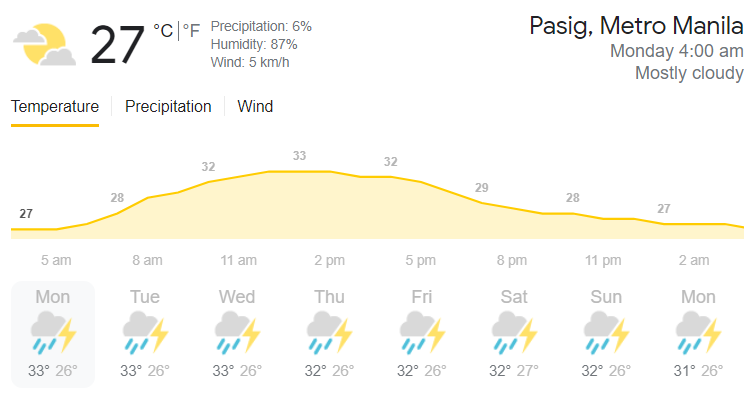
\includegraphics{./del.png}
\caption{Google's Weather Forecast}
\end{figure}

\textbf{Reference}

IBM Business. (2021, July 12). Maybunga, Philippines Weather Forecast
and Conditions - The Weather Channel. The Weather Channel.
\url{https://weather.com/weather/today/l/14.58,121.09?par=google}.

\begin{center}\rule{0.5\linewidth}{0.5pt}\end{center}

\begin{center}\rule{0.5\linewidth}{0.5pt}\end{center}

\end{document}
